\section{Analysis of the Model}
\label{sec:fault_analysis_2}
In this section we describe results from the nominal model analysis and the fault analysis.  

\subsection{Nominal Model Analysis}
\label{subsec:nominalAnalysis}
Before performing fault analysis, users should first check that the safety properties are satisfied by the nominal design model. This analysis can be performed monolithically or compositionally in \gls{agree}. Using monolithic analysis, the contracts at all levels of the architecture are flattened and used in the proof of the top-level safety properties of the system. Compositional analysis, on the other hand, will perform the proof layer by layer top down, essentially breaking the larger proof into smaller problems. A more comprehensive description of these types of proofs and analyses is found in~\cite{NFM2012:CoGaMiWhLaLu,QFCS15:backes} 

The \gls{wbs} has a total of 13 safety properties at the top level that are supported by subcomponent assumptions and guarantees, shown in Table \ref{tab:safetyProperties}. Since there are 8 wheels, contract S18-WBS-0325-wheelX is repeated 8 times, one for each wheel. The system includes both left (L) and right (R) side braking, so S18-WBS-R/L-0322 occurs twice. The behavioral model in total consists of 36 assumptions and 246 supporting guarantees.

%\vspace{-0.2cm}
\begin{center}
\begin{table}
\caption{Safety Properties of WBS}
\begin{tabular}{@{}ll}
\toprule
\textbf{S18-WBS-R-0321} \\Loss of all wheel braking during landing or RTO shall be less than $5.0 \times 10^{-7}$ per flight.                                    \\ \midrule 
\textbf{S18-WBS-R/L-0322}  \\ Asymmetrical loss of wheel braking (Left/Right) shall be less than $5.0 \times 10^{-7}$ per flight. \\ \midrule
\textbf{S18-WBS-0323} \\ Never inadvertent braking with all wheels locked shall be less than $1.0 \times 10^{-9}$ per takeoff.                                                                                                                                                                                                               \\ \midrule
\textbf{S18-WBS-0324}  \\ Never inadvertent braking with all wheels shall be less than $1.0 \times 10^{-9}$ per takeoff.                                                                                                            \\ \midrule
\textbf{S18-WBS-0325-wheelX} \\ Never inadvertent braking of wheel X shall be less than $1.0 \times 10^{-9}$ per takeoff.                                                                                                           .                                                                                                                 \\ \bottomrule
\end{tabular}
\vspace{0.4cm}
%\caption{Safety Properties of WBS}
\label{tab:safetyProperties}
\end{table} 
\end{center} 
%\vspace{-2cm}

\subsection{Fault Model Analysis}
In Section~\ref{sec:fault_modeling}, we outlined the system and its corresponding model. This section describes the analysis of the fault model described in Subsections ~\ref{subsec:compFM} --~\ref{subsec:analysisStmts}. There are two main options for fault model analysis using the Safety Annex. The first option injects faulty behavior allowed by the faulty hypothesis (Subsection~\ref{subsec:analysisStmts}) into the \gls{agree} model and returns this fault annotated Lustre program to JKind for analysis. JKind is an open-source industrial infinite-state inductive model checker for safety properties and runs all back-end analysis for \gls{agree}~\cite{2017arXiv171201222G} as described in Section~\ref{sec:implementation}. The injection of faulty behavior into the \gls{agree} model allows for the activity of faults within the model and traceability information provides a way for users to view a counterexample to a violated contract in the presence of faults. 

The second option for analysis is used to generate minimal cut sets for the model. The path from the user written fault model to JKind is the same in both kinds of analysis, but the fault annotations specify which results to compute and display to the user.  

\subsubsection{Verification in the Presence of Faults: Max N Analysis}
Using a max number of faults for the hypothesis, the user can constrain the number of simultaneously active faults in the model. The faults are added to the \gls{agree} model for the verification and the model checker attempts to prove the top level properties given these constraints. If this cannot be done, a counterexample is generated showing which of the faults (N or fewer) are active and which contracts are violated. 

The user can choose to perform either compositional or monolithic analysis using a max N fault hypothesis. In compositional analysis, the analysis proceeds in a top down fashion, from one level (or layer) of the model to the next. To prove upper layer properties, the properties in the layer directly beneath that level are used to perform the proof. Users constrain the maximum number of faults within each layer of the model by specifying the maximum fault hypothesis statement to that layer. If any lower level property failed due to activation of faults, the property verification at the higher level can no longer be trusted because the higher level properties were proved based on the assumption that the direct sub-level contracts are valid. This form of analysis is helpful to see weaknesses in a given layer of the system.  

In monolithic analysis the layers of the model are flattened, which allows a direct correspondence between all faults in the model and their effects on the top level properties. As with compositional analysis, a counterexample shows these N or less active faults. 

\subsubsection{Verification in the Presence of Faults: Probabilistic Analysis} 
Given a probabilistic fault hypothesis, this corresponds to performing analysis with the combinations of faults whose simultaneous occurrence probability is less than the probability threshold. This is done by inserting assertions that allow those combinations in the Lustre code. If the model checker proves that the safety properties can be violated with any of those combinations, one of such combination will be shown in the counterexample. This form of analysis is not performed using a probabilistic model checker, but rather probabilistic computations are performed after behavioral analysis is complete. 
% Probabilistic analysis done in this way must use the monolithic AGREE option.

It is assumed that the faults occur independently and possible combinations of faults are computed and passed to the Lustre model to be checked by the model checker. As seen in Algorithm 1, the computation first removes all faults from consideration that are too unlikely given the probability threshold. The remaining faults are arranged in a priority queue $\mathcal{Q}$ from high to low. Assuming independence in the set of faults, we take a fault with highest probability from the queue (step 5) and attempt to combine the remainder of the faults in $\mathcal{R}$ (step 7). If this combination is lower than the threshold (step 8), then we do not take into consideration this set of faults and instead remove the tail of the remaining faults in $\mathcal{R}$. In this calculation, we assume independence among the faults. 
 
\begin{algorithm}[H]
	% \KwData{this text}
	% \KwResult{how to write algorithm with \LaTeX2e }
	$\mathcal{F} = \{\}$ : fault combinations above threshold \;
	$\mathcal{Q}$ : faults, $q_i$, arranged with probability high to low \;
	$\mathcal{R} = \mathcal{Q}$ , with $r \in \mathcal{R}$\;
	\While{$\mathcal{Q} \neq \{\} \land \mathcal{R} \neq \{\}$ }{
		$q =$ removeTopElement($\mathcal{Q}$) \;
		\For{$i=0:|\mathcal{R}|$}{
			$prob = q \times r_i$ \;
			\eIf{prob $<$ threshold}{
				removeTail($\mathcal{R}, j=i:|\mathcal{R}|$)\;
			}{
				add($\{q, r_i\}, \mathcal{Q}$)\;
				add($\{q, r_i\}, \mathcal{F}$)\;
			} % end if else
		} % end for
	} % end while
	\caption{Monolithic Probability Analysis}
	\label{alg:prob_monolithic}
\end{algorithm}


\subsubsection{Generate Minimal Cut Sets: Max N Analysis }
\label{sec:maxN_generate}
Generation of minimal cut sets was performed on the Wheel Brake System and results are shown in Table~\ref{tab:wbs_maxN_results}. Notice in Table~\ref{tab:wbs_maxN_results}, the label across the top row refers to the cardinality (\textit{n}) and the corresponding column shows how many cut sets are generated of that cardinality. When the analysis is run, the user specifies the value \textit{n}. This gives cut sets of cardinality less than or equal to \textit{n}. Table~\ref{tab:wbs_maxN_results} shows the total number of cut sets of cardinality \textit{n}. The total number of cut sets computed at the given threshold is the sum across a row. (For the full text of the properties, see Table~\ref{tab:safetyProperties}.) 


\begin{table}[htbp]
\begin{center}
\caption{WBS Minimal Cut Set Results for Max \textit{n} Hypothesis}
    \begin{tabular}{ | l | l | l | l | l | l |}
    \hline
    \textbf{Property} & $\bm{n = 1}$ & $\bm{n = 2}$ & $\bm{n = 3}$ & $\bm{n = 4}$ 
		& $\bm{n = 5}$    \\ \hline \hline
    0321 & 7 & 0 & 0 & 256 & 57,600   \\ \hline
    0322-R & 75 & 0 & 0 & 0 & 0  \\ \hline
    0322-L & 75 & 0 & 0 & 0 & 0  \\ \hline
    0323 & 182 & 0 & 0 & 0 & 0  \\ \hline
    0324 & 8 & 3,665 & 28,694 & 883,981 & - \\ \hline
    0325-WX & 33 & 0 & 0 &0 &0 \\ \hline
    \end{tabular}
    \label{tab:wbs_maxN_results}
    \end{center}
\end{table}

As can be seen in Table~\ref{tab:wbs_maxN_results}, the number of cut sets increases proportional to the cardinality of the cut sets. Intuitively, this can be understood as simple combinations of faults that can violate the hazard; if more things go wrong in a system at the same time, the more likely a property will be violated. Property S18-WBS-0324 with a max fault hypothesis of 5 was unable to finish due to an out of memory error. At the time that the error was thrown, the number of cut sets exceeded 1.5 million. In practice, it is impossible to manually sift through multiple thousands of cut sets, but an analyst will instead filter out the combinations that are sufficiently unlikely to occur based on a truncation limit. In the next subsection (Generate Minimal Cut Sets: Probabilistic Analysis), we discuss the use of a truncation limit through probabilistic analysis. The probabilistic approach presents more realistic and useful number of cut sets for consideration.

\subsubsection{Generate Minimal Cut Sets: Probabilistic Analysis}
\label{sec:prob_generate}
Both probabilistic analysis and max $n$ analysis use the same underlying minimal cut set generation algorithm (see Section~\ref{sec:implementation}), but in probabilistic analysis the minimal cut sets are pruned to include only those fault combinations whose probability of simultaneous occurrence exceed the given threshold in the hypothesis. 

The probabilistic analysis for the WBS was given a top level threshold per property as stated in AIR6110 and shown in Table~\ref{tab:safetyProperties}. The faults associated with various components were all given probability of occurrence according to the AIR6110 document~\cite{AIR6110}. The table shows the property name and associated probability. The generation of minimal cut sets provided all sets that violate that property whose combined probabilities (assuming independence) are greater than the threshold. The number of sets per cardinality are listed in the table. 

\begin{table}[htbp]
\begin{center}
\caption{WBS Minimal Cut Set Results for Probabilistic Hypotheses}
    \begin{tabular}{ | l | l | l | l | l | l | l | }
    \hline
    \textbf{Property} & $n=1$ & $n=2$ & $n=3$ & $n=4$ 
		& $n=5$    \\ \hline \hline
    0321: $5.0 \times 10^{-7}$ & 7 & 0 & 0 & 256 & 0   \\ \hline
    0322-R: $5.0 \times 10^{-7}$ & 75 & 0 & 0 &0 &0   \\ \hline
    0322-L: $5.0 \times 10^{-7}$ & 75 & 0 & 0 & 0 & 0    \\ \hline
    0323: $1.0 \times 10^{-9}$ & 182 & 0 & 0 & 0 & 0    \\ \hline
    0324: $1.0 \times 10^{-9}$ & 8 & 3665 & 0 & 0 & 0   \\ \hline
    0325-W1: $1.0 \times 10^{-9}$ & 33 & 0 & 0 &0 &0    \\ \hline
    \end{tabular}
    \label{tab:wbs_prob_results}
    \end{center}
\end{table}

As shown in Table~\ref{tab:wbs_prob_results}, the number of allowable combinations drops considerably when given probabilistic threshold as compared to just fault combinations of certain cardinalities. For example, one contract (inadvertent wheel braking of all wheels) had over a million minimal cut sets produced when looking at it in terms of max N analysis, but after taking probabilities into account, it is seen on Table~\ref{tab:wbs_prob_results} that the likely contributors to a hazard are minimal cut sets of cardinality one. The probabilistic analysis eliminated many thousands of cut sets from consideration.

In Table~\ref{tab:wbs_prob_results}, the property 0321 has a truncation limit of $1.0 \times 10^{-9}$ with 8 single points of failure. If this property has a catastrophic classification, these single points of failure must be eliminated. Likewise with cut sets of cardinality n = 2, there are a total of 3665 combinations that a safety analyst must manually examine. Within this analysis framework, there are multiple ways to address the number of cut sets. One is to re-examine how the faults are modeled (e.g., consolidate a valve's two failure modes into one as fail-open and fail-closed cannot occur the same time) and another is to re-evaluate the design of the model which is discussed in detail in an upcoming subsection (Use of Analysis Results to Drive Design Change). 

\subsubsection{Analysis Result Representations of Minimal Cut Sets}
Results from Generate Minimal Cut Sets analysis can be represented in one of the following forms.
\begin{enumerate}
\item The minimal cut sets can be presented in text form with the total number per property, cardinality of each, and description strings showing the property and fault information. A sample of this output is shown in Figure~\ref{fig:detailedMCS}. 

\begin{figure}[h!]
	%\hspace*{-2cm}
	%\vspace{-0.1in} 
	\begin{centering}
		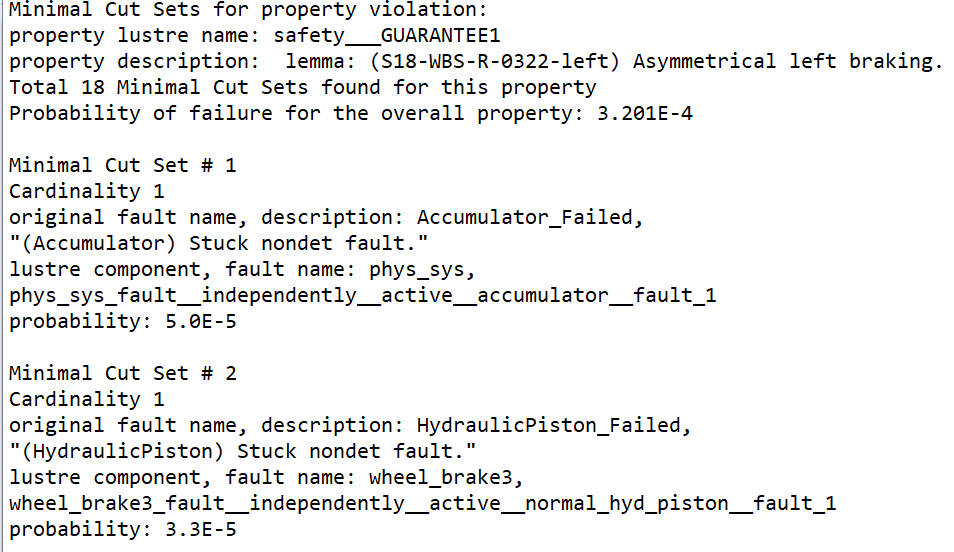
\includegraphics[width=0.9\textwidth]{images/mcs_detailed.png}
	\caption{Detailed Output of MinCutSets}
		\label{fig:detailedMCS}
	\end{centering}
\end{figure}

\item The minimal cut set information can be presented in tally form. This does not contain the fault information in detail, but instead gives only the tally of cut sets per property. This is useful in large models with many cut sets as it reduces the size of the text file. An example of this output type is seen in Figure~\ref{fig:tallyMCS}.

\begin{figure}[h!]
	%\hspace*{-2cm}
	%\vspace{-0.5in} 
	\begin{centering}
		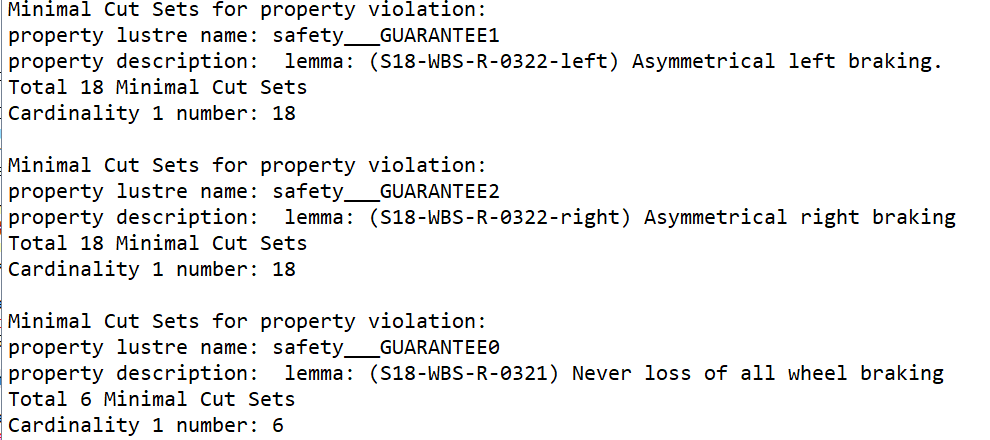
\includegraphics[width=0.75\textwidth]{images/mcs_tally.png}
	\caption{Tally Output of MinCutSets}
		\label{fig:tallyMCS}
	\end{centering}
\end{figure}

The minimal cut sets produced by this analysis are combinations of faults; permutations of the faults in terms of exposure time and order of occurrence are not part of the results of this analysis. We aim to address this limitation in future work (see Section~\ref{sec:conclusion}).


\end{enumerate}

\subsubsection{Use of Analysis Results to Drive Design Change}
\label{sec:designchange}
We use a single top level requirement of the \gls{wbs} to illustrate how Safety Annex can be used to detect design flaws and how faults can affect the behavior of the system (S18-WBS-0323 : Never inadvertent braking with all wheels locked). This safety property description can be found in detail in Section \ref{sec:fault_modeling}. Upon running max $n$ compositional fault analysis with $n = 1$, this particular fault was shown to be a single point of failure for this safety property. A counterexample is shown in Figure \ref{fig:counterexample} showing the active fault on the pedal sensor. 

\begin{figure}[h!]
	%\vspace{-0.2in}
	\begin{centering}
		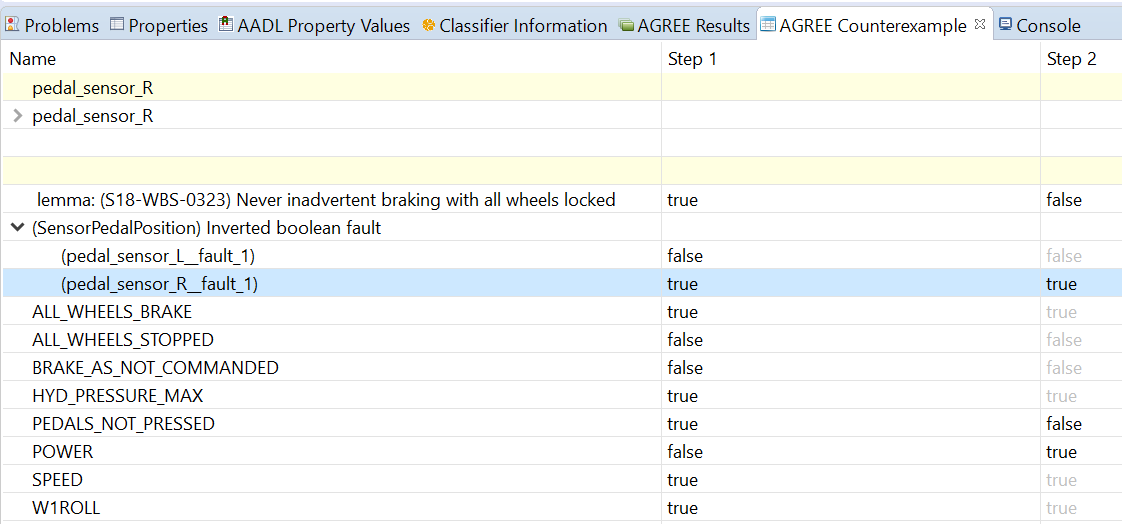
\includegraphics[width=\textwidth]{images/counterexample.png}
	%\vspace{-0.3in}
	\caption{AGREE counterexample for inadvertent braking safety property}
	\label{fig:counterexample}
	%\vspace{-0.2in}
	\end{centering}
\end{figure} 

To mitigate this problem, redundancy can be added to handle a single  faulty sensor by using three sensors. The overall output from the sensor system may use a voting scheme to determine validity of the sensor reading. There are multiple voting schemes that are possible, one of which is a majority voting. 
When three sensors are present, this mitigates the single point of failure problem. New behavioral contracts are added to the sensor system to model the behavior of redundancy and voting. 
%\end{itemize}

In the case of the pedal sensor in the \gls{wbs}, the latter of the two strategies outlined above was implemented. A sensor system was added to the model which held three pedal sensors. The output of this subsystem was constrained using a majority voting scheme. Upon subsequent runs of the analysis (regardless which type of run was used), resilience was confirmed in the system regarding the failure of a single pedal sensor. Figure \ref{fig:sensorsystem} outlines these architectural changes that were made in the model.

\begin{figure}[h!]
	%\vspace{-0.2in}
	\begin{centering}
		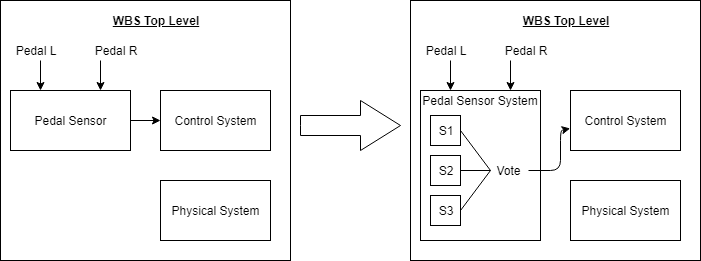
\includegraphics[width=0.9\textwidth]{images/sensorsystem.png}
	%\vspace{-0.3in}
	\caption{Changes in the architectural model for fault mitigation}
	\label{fig:sensorsystem}
	%\vspace{-0.2in}
	\end{centering}
\end{figure}

As can be seen through this single example, a system as large as the \gls{wbs} would benefit from many iterations of this process. Furthermore, if the model is changed even slightly on the system development side, it would automatically impact the safety analysis and any negative outcomes would be shown upon subsequent analysis runs. This effectively eliminates any miscommunications between the system development and analysis teams and creates a new safeguard regarding model changes. 

For more information on types of fault models that can be created as well as details on analysis results, see the users guide located in the GitHub repository \cite{SAGithub}. This repository also contains all models used in this project. 


